\documentclass[tikz,border=8pt]{standalone}
% Shared look for every TikZ diagram. Load with \input{../../tools/tikz-style.tex}
\usepackage[sfdefault]{roboto}
\usetikzlibrary{arrows.meta, positioning, shapes.geometric, calc, fit, backgrounds}
\definecolor{cblue}{HTML}{4C78A8}
\definecolor{corange}{HTML}{F58518}
\definecolor{cgreen}{HTML}{54A24B}
\definecolor{cred}{HTML}{E45756}
\definecolor{cpurple}{HTML}{B279A2}
\definecolor{cgrey}{HTML}{6B6B6B}
\tikzset{
  every picture/.style={font=\sffamily, line width=1.2pt},
  box/.style={draw=#1, fill=#1!12, rounded corners=4pt, align=center, inner sep=7pt, minimum height=1.1cm},
  box/.default=cgrey,
  arrow/.style={-{Stealth[length=3mm]}, draw=cgrey, line width=1.4pt},
  title/.style={font=\sffamily\bfseries\Large},
  note/.style={font=\sffamily\small, text=cgrey, align=center},
}
\AtBeginDocument{\hyphenpenalty=10000 \exhyphenpenalty=10000}

% Stanley on the 10 m arc once settled: the front axle stays on the course (radius 10 m about the arc's centre),
% so the rear axle, 2.5 m behind it and square to its own circle, runs on a circle of radius sqrt(10^2 - 2.5^2)
% = 9.682 m: 0.318 m inside the course. Drawn with the rear axle at -60 deg about the centre: rear (4.841, -8.385),
% heading 30 deg, front (7.006, -7.135); the front wheel points along the course, 44.48 deg, so the steering is
% 14.48 deg. Origin at the arc's centre (off the picture, up and to the left); 1 unit = 1 m.
\begin{document}
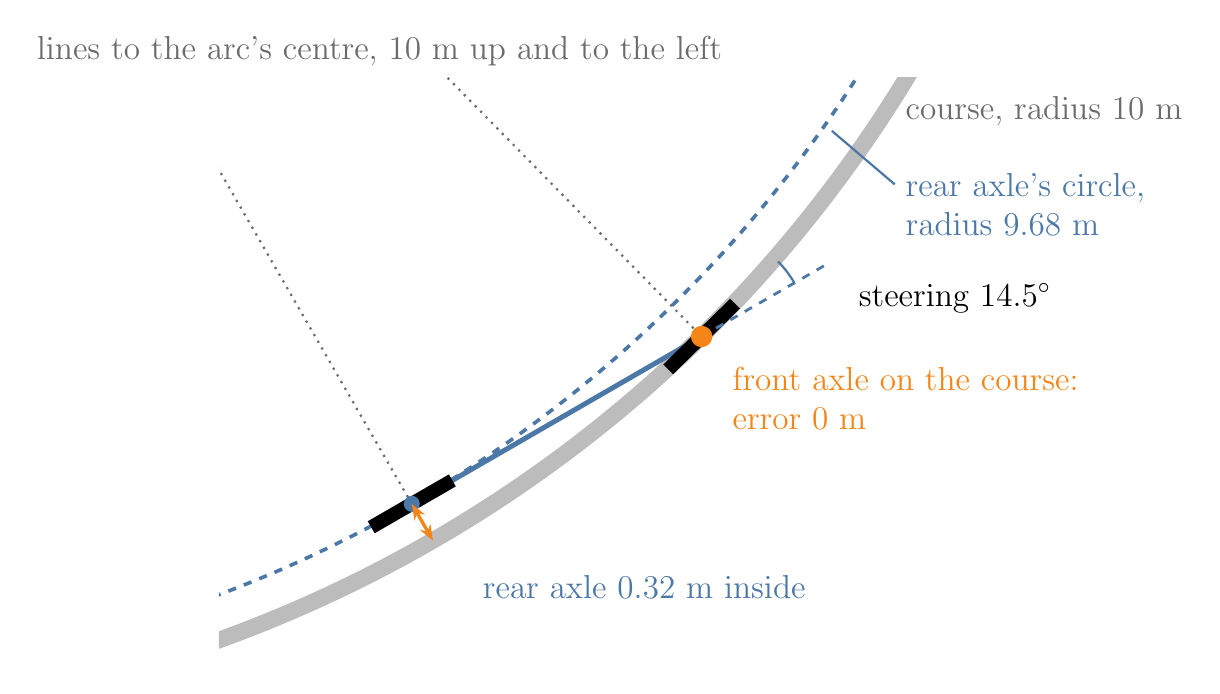
\begin{tikzpicture}[scale=1.7, every node/.append style={font=\large}]
  \coordinate (Rr) at (4.841,-8.385);
  \coordinate (F) at (7.006,-7.135);
  \begin{scope}
    \clip (3.4,-9.6) rectangle (9.0,-5.2);
    \draw[cgrey!45, line width=6pt] (0,0) ++(-80:10) arc[start angle=-80, end angle=-25, radius=10];
    \draw[cblue, dashed, line width=1.3pt] (0,0) ++(-80:9.682) arc[start angle=-80, end angle=-25, radius=9.682];
    \draw[cgrey, line width=0.8pt, dotted] (0,0) -- (F);
    \draw[cgrey, line width=0.8pt, dotted] (0,0) -- (Rr);
  \end{scope}
  \node[cgrey, anchor=west] at (8.45,-5.45) {course, radius 10 m};
  \node[cblue, anchor=west, align=left] at (8.45,-6.15) {rear axle's circle,\\radius 9.68 m}; \draw[cblue, line width=0.8pt] (8.45,-6.0) -- (7.98,-5.6);
  \node[cgrey, anchor=south, align=center] at (4.6,-5.2) {lines to the arc's centre, 10 m up and to the left};
  % the car
  \draw[cblue, line width=1.8pt] (Rr) -- (F);
  \draw[black, line width=5pt] ($(Rr)+(30:-0.35)$) -- ($(Rr)+(30:0.35)$);
  \draw[black, line width=5pt] ($(F)+(44.48:-0.35)$) -- ($(F)+(44.48:0.35)$);
  \draw[cblue, dashed, line width=1pt] (F) -- ++(30:1.1);
  \draw[cblue, line width=0.8pt] ($(F)+(30:0.8)$) arc[start angle=30, end angle=44.48, radius=0.8];
  \node[black, anchor=west] at (8.1,-6.85) {steering $14.5^\circ$};
  \fill[cblue] (Rr) circle (0.06); \fill[corange] (F) circle (0.08);
  \node[corange, anchor=north west, align=left] at ($(F)+(0.15,-0.15)$) {front axle on the course:\\error 0 m};
  % the 0.32 m gap at the rear axle
  \draw[corange, line width=1.2pt, {Stealth[length=2mm]}-{Stealth[length=2mm]}] (Rr) -- ($(Rr)+(-60:0.318)$);
  \node[cblue, anchor=north west, align=left] at ($(Rr)+(0.45,-0.45)$) {rear axle 0.32 m inside};
\end{tikzpicture}
\end{document}
